%%%%%%%%%%%%%%%%%%%%%%%%%%%%%%%%%%%%%%%%%%%%%%%%%%%%%%%%%%%
% Chapter 2
\chapter{Background and Literature Review}

\begin{singlespacing}
\begin{microabstract}
    This chapter presents fundamental background information and concepts used in this thesis along with relevant literature review. The reader is presented with the role of machine learning in finance and the need for it. The chapter then compares and contrasts Classical versus Bayesian machine learning. A detailed introduction to the hidden Markov model is provided along with selected applications and learning methods utilising the expectation-maximisation algorithm. Finally, artificial neural networks are introduced along with some applications. Feed-forward neural networks are discussed along with their architecture, layout and learning method.
\end{microabstract}
\end{singlespacing} 

\section{Machine learning in finance}\label{Ch2Sec1}

Finance falls in the optimal spot for machine learning. Compared to many other sectors, this is a sector where transactional data is plentiful, where data is systematically captured (particularly in recent years due to increased regulatory requirements) and where there are many complex interrelationships across multiple variables that lend themselves to more sophisticated analytical techniques. And yet, machine learning is at its relative infancy in this sector.

In a recent research study by MIT Sloane Management Review and the Boston Consulting Group~\autocite{ransbotham2017reshaping}, more than 3,000 senior business executives, managers and analysts from different sectors were surveyed across the globe on the expected impact of AI on their sector. Whilst all sectors have high expectations of AI, the Finance sector has the biggest gap between current and future states -- i.e., the sector with the greatest potential relative to where they are today (refer to Figure~\ref{Ch2Fig:1}). This has likely been driven by the historical emphasis of banks on personal relationships to drive sales, banks having legacy infrastructure/practices, and banks being generally slow to adopt some of the new technologies.

\begin{figure}[!ht]\centering
\includegraphics[width=0.6\linewidth]{./figures/Ch1fig1.pdf}
\caption{Expectations for AI's effect on businesses' offerings in 5 years time~\autocite{ransbotham2017reshaping}}\label{Ch2Fig:1}
\end{figure}

Still, digitisation has been evolving the sector, laying the ground for machine learning. Over the past two decades, the front offices (sales and trading functions) of banks have seen extensive digital transformation. Digital channels have become one of the primary ways to access a bank’s offerings and people -- either through banks' or third-party platforms to view and request price quotes or to execute transactions digitally.


Now, the time is right for banks to take digitisation to the next level -- to leverage machine learning to bring differentiated insight and intelligence that can generate enhanced revenues. In Fixed income commodities and currencies (FICC), which is the area of focus of this research, there are several business drivers to this change~\autocite{MckinseyCompany}:

\begin{description}
    \item[Lack of differentiation.]\strut\\ Whilst almost all banks have launched digital offerings, many have failed to build distinctive propositions. As an example, most trading platforms offered by banks have similar capabilities (and largely similar functionalities) and are different only by look-and-feel. Also, the propositions often on these platforms do not tend to be particularly innovative -- they are mostly offline offerings being moved online and often do not create fundamentally different revenue streams.
    \item[Misunderstood economics of electronification.]\strut\\ Many digital investments made by banks (some in the tune of \$100m or more) have simply not paid back, partly due to the lack of differentiation mentioned above. Further, clients often use digital channels as ‘shop windows’ and continue making transactions through voice channels, meaning that digital channels become loss leaders due to hefty digital spend. Electronification has compressed margins without bringing in the increase in volumes expected.
    \item[Declining foreign exchange trade volumes.]\strut\\ For the first time since 2001, global foreign exchange (FX) trading volumes have declined between two consecutive surveys conducted by the Bank for International Settlements (BIS). Global FX turnover was reported to have fallen \$300billion (almost 6\%) from \$5.4 trillion (April 2013) to \$5.1 trillion (April 2016) transactions per day~\autocite{moore2016downsized}. Figure~\ref{Ch2Fig:2} below depicts FX turnover volume broken down by instruments (swaps, spots, forwards, options and other derivatives). This has further put pressure on banks to find more differentiated ways to generate revenues in a shrinking market.
\end{description}

      
\begin{figure}[!htb]\centering
\includegraphics[width=0.6\linewidth]{./figures/Ch1fig2.pdf}
\caption{Turnover by Instrument~\autocite{moore2016downsized}}\label{Ch2Fig:2}
\end{figure}

Within this market context, there is now significant investment being poured into data analytics and innovation in financial institutions. Many have started to set-up Data/AI innovation groups labs in the past 2-3 years (for example BAML's Data and Innovation Group and BNP Paribas's Data Lab) as well as starting to persist eFX-data in databases.

\section{Classical versus Bayesian machine learning}\label{Sec:CvsB}

\textcolor{red}{TODO:}  think about adding something from JS slide img\_8023.jpg

\subsection{Probability and statistics}

First and foremost it is important to point out the difference between probability and statistics no matter how trivial that may seem. Probability is a self-contained mathematical discipline and probabilistic reasoning uses probabilistic models, which strictly obey the probability axioms \autocite{kolmogorov2018foundations}. Statistics is more of an art, where for any given problem there may exist several plausible methods, which give a different answer \autocite{bertsekas2002introduction}. This distinction is important as machine learning is based on statistics and statistical learning theory. Tibshirani et al \autocite{james2013introduction} describe statistical learning as ``a vast set of tools for understanding data and these tools can be classified as supervised or unsupervised''.

\subsection{Classical versus Bayesian statistics}
If you are a machine learner, the chances are that you would be aware of the 250-year old debate between Classicists (also called frequentists) and the Bayesians. They form two distinct competing camps when it comes to the approach and philosophy of statistical inference (decision making). Broadly speaking, Bayesian statistics dominated \nth{19} century statistical practice, while the \nth{20} century was more classicist \autocite{efron2005bayesians} The fundamental difference is on how they handle unknown models or variables. Bayesians treat model parameters as random variables with known distributions, whereas the classicists treat them as deterministic quantities, which happen to be unknown \autocite{bertsekas2002introduction}.

A classicist's version of probability is defined as the long-term frequency of an observation or measurement. The classicists believe in a single truth. They claim the more data they collect the more accurately they can predict the truth. For example in a coin flipping experiment, the classicists would perform repeated flips to see if the long-term frequency is heads or tails, with the long-term frequency eventually tending to the truth \autocite{ambaum2012frequentist}

Bayesians on the other hand define probability as the plausibility of a hypothesis given an incomplete and subjective knowledge. Bayesians are not seeking a single truth via data collection. Bayesians use data as evidence for particular hypothesis. If a Bayesian were to flip a coin, they would simply observe a number of flips and then use this information to make deductions about the fairness of the coin \autocite{ambaum2012frequentist}

The Bayesians and Classicist each have a different interpretation of probability. If we take the example of flipping a fair coin, commonly we say the probability of obtaining a tails in 0.5. The classicists view probability as long run frequencies of events. In the coin flip example, they would think if we flip the coin many times, we expect it to land tails half the time \autocite{murphy2012machine}. Whereas Bayesians use probability to quantify uncertainly about something, therefore it is fundamentally related to information and not repeated trials. With regards to the coin flip, Bayesians believe the coin is equally likely to land heads or tails on the next flip.

Many machine-learning problems are well suited to the Bayesian philosophy particularly where we need to model uncertainty around events, which do not have long-term frequencies. For example, will the Antarctic ice sheet melt in the next 20 years? Or we observe a blip on a radar screen and we want to compute the probability distribution over the location of the corresponding target (e.g. a missile) \autocite{barberBRML2012}. In both of these examples the classical approach falls short as the idea of repeated trials does not make sense. Table~\ref{Ch2Tab:1} provides a brief comparison of the Bayesian versus Classical philosophy.


\begin{table}[!ht]\centering\footnotesize
    \caption{Bayesian and classical methods compared and contrasted}\label{Ch2Tab:1}
    \begin{tabular}{
        >{\raggedright\arraybackslash}p{0.5\linewidth-2\tabcolsep}
        >{\raggedright\arraybackslash}p{0.5\linewidth-2\tabcolsep}
        }
        \toprule
        \textbf{Bayesian} & \textbf{Classical} \\
        \midrule
        The fairness of a flipped coin is answered by a probability distribution. It is not a fixed value and it is the experimenter's subjective perception. For example: $p\left( \text{coin} = H|\text{Data} \right)$
        &
        The fairness of a flipped coin is answered by a single value, which would be the inherent property of the coin. Thus everyone should arrive at the same answer. For example $p\left( \text{coin}=H \right) = 0.5$
        \\
        \midrule
        In the coin flipping case, as you feed more data into your model the distribution $p\left( \text{coin}=H|Data \right)$ tightens around the `true' value of 0.5
        &
        As you feed more data into your model your confidence interval tightens around the `true' value of 0.5
        \\
        \midrule
        Computationally intensive, but having a renaissance with more computing power. It requires sampling methods for all but a small family of distributions.
        &
        Less computationally intensive than the Bayesian approach.
        \\
        \midrule
        Missing data are a common problem and Bayesians are able to deal with this by summing out variables.
        &
        All missing data must be provided for when multiplying matrices by using for example interpolation.
        \\
        \midrule
        Common practice in \nth{19} Century.
        &
        Common practice in \nth{20} Century.
        \\
        \midrule
        Unknown parameters are treated as random variables with known prior distributions
        &
        Unknown parameters are treated as constants to be determined
        \\
        \midrule
        Requires knowledge or construction of a `subjective prior'.
        &
        Does not require a prior.
        \\
        \midrule
        Relies on presenting presents density graphs of posterior distributions.
        &
        Relies on presenting p-values and confidence intervals.
        \\
        \midrule
        The main inference method is maximum a posteriori (MAP).
        &
        The main inference method is maximum likelihood (ML).
        \\
        \midrule
        Returns parameter estimates which are close to the true parameter values in a probabilistic sense.
        &
        Returns parameter estimates which are nearly correct under any possible value of unknown parameter.
        \\
        \midrule
        The classical confidence interval is equivalent to probability mass distribution between two values.
        &
        Unable to reject Null Hypothesis to establish likelihood of fair coin at the desired confidence interval e.g 95\%
        \\
        \bottomrule
  \end{tabular}
\end{table}


\subsection{Bayes' Theorem}

The driving force of Bayesian machine learning is Bayes' Theorem. We first present a brief recap of Bayes' Theorem (also referred to as Bayes' rule or Bayes' Law). Named after the English statistician Thomas Bayes (1702--1761) Bayes' rule is a statement of conditional probabilities, and plays a pivotal role in probabilistic reasoning, it is simply derived as follows. As D Barber \autocite{barberBRML2012} points out the rules of probability combined with Bayes' rule make it a complete reasoning system.

The probability of an event $A$ given another event $B$ ($A$ conditioned on knowing $B$) is expressed as the conditional probability expression:
\begin{equation}\label{Ch3Eq0}
    p\left( A|B \right)
\end{equation}

It can further be shown that the above conditional probability can be expressed as:
\begin{align}
    p\left( A|B \right) & = \dfrac{p \left( A\text{ and }B \right)}{p\left( B \right)} = \dfrac{p\left( A,B \right)}{p\left( B \right)} \label{Ch3Eq1}\\
    &\strut\nonumber\\
    p\left( B|A \right) & = \dfrac{p \left( A\text{ and }B \right)}{p\left( A \right)} = \dfrac{p\left( A,B \right)}{p\left( B \right)} \label{Ch3Eq2}
\end{align}

Re-arranging equations~(\ref{Ch3Eq1}) and~(\ref{Ch3Eq2}):
\begin{align}
    p\left( A,B \right) & = p\left( A|B \right) \cdot p\left( B \right) \label{Ch3Eq3}\\
    &\strut\nonumber\\
    p\left( B,A \right) & = p\left( B|A \right) \cdot p\left( A \right) \label{Ch3Eq4}
\end{align}

Equating the right hand sides of expressions~\ref{Ch3Eq3} and \ref{Ch3Eq4} we arrive at Bayes' rule:
\begin{equation}
    \overbrace{p\left( A|B \right)}^{\text{posterior}} =
    \dfrac
        {
        \overbrace{p\left( B|A \right)}^{\text{likelihood}}
        \overbrace{p\left( A \right)}^{\text{prior}}
        }
        {\underbrace{p\left( B \right)}_{\text{evidence}}}
\end{equation}

Bayes' rule shows how from a generative model $p\left( B|A \right)$ of the dataset plus your prior (initial) belief/knowledge $p\left( A \right)$ about the most appropriate variable values before any evidence is taken into account, one can infer the posterior distribution $p\left( A|B \right)$ of the variable given the observed data.

The most probable posterior is known as the maximum a posteriori probability (MAP). This is a setting which maximises the posterior, i.e.:
\begin{equation}
    A_* = \argmax_A p\left( A|B \right)
\end{equation}

In the case of a flat prior i.e. when $p\left( A \right)$ is constant with respect to $A$, the MAP solution is equivalent to the maximum likelihood, i.e. the $A$ that maximises the likelihood $p\left( B|A \right)$ of the model generating the observed data \autocite{barberBRML2012}. The posterior distribution is what we infer in light of the observed data. It is the probability that $A$ is true after considering the data.

The steps involved in Bayes' rule are better explained using the simple example of smoking and lung cancer with the aid of a Venn diagram (Figure~\ref{Ch2Fig:3}).

\begin{figure}[!ht]\centering
    \strut\\
    \begin{tikzpicture}[x=1cm,y=1cm]
        \draw (-2,-2) coordinate(BL) rectangle (3,2.5) coordinate (TR);
        \node[below right] (S) at (BL|-TR) {$\Omega=1$million};
        \fill[COL2,draw=black] (0,0) coordinate(A) circle (1.0);
        \path (A)--++(225:1) coordinate[at end] (a);
        \draw (a)--++(225:5pt) node[at end,anchor=45,inner sep=1pt] {$C$};
        \path (A) --++(180:1) coordinate[at end] (An);
        \fill[COL1,draw=black] (1,0)  coordinate(B) circle (1.5);
        \path (B)--++(305:1.5) coordinate[at end] (b);
        \draw (b)--++(305:5pt) node[at end,anchor=135,inner sep=1pt] {$S$};
        \path (B) --++(130:1.5) coordinate[at end] (Bn);
        \path ($(A)!0.25!(B)$) coordinate (C1) --++(270:1.5) coordinate (C2);

        \begin{scope}
            \clip (1,0)  circle (1.5);
            \fill[COL3,draw=black] (0,0) circle (1);
        \end{scope}

        \begin{scope}[every node/.style={at end,above right,font=\footnotesize,inner sep=1pt}]
            \draw (S) --++(180:9) coordinate(X) node {\strut Sample Space (e.g 1 million)};
            \draw (Bn) --(Bn-|X) node {\strut Event $S$: People who smoke};
            \draw (C1)--(C2) --(C2-|X) node {\strut Event $C\cap S$: Smokers who have lung cancer};
            \draw (An) --(An-|X) node {\strut Event $C$: People with lung cancer};
        \end{scope}

    \end{tikzpicture}
    \caption{Venn diagram of smoking and lung cancer}\label{Ch2Fig:3}
\end{figure}


In Figure~\ref{Ch2Fig:3} $p\left( C|S \right)$ represents the probability you that have lung cancer given that you are a smoker, which is not trivial to ascertain. The likelihood $p\left( S|C \right)$ is the flip side of the posterior distribution. This is the evidence about $C$ provided by the data $S$.

In our example $p\left( S|C \right)$ the probability of being a smoker given that the person has lung cancer. One could easily measure this by interviewing people with lung cancer and collecting the data.

The prior $p\left( C \right)$ is an initial belief probability that $C$ is true prior to considering the data i.e. the probability of having lung cancer.

The evidence $p\left( S \right)$ is known as the marginal likelihood or the normalisation constant. This can also be thought of as the total probability taking everything into account. In our example it would equate to the probability of being a smoker.

In further support of the Bayesian framework, as D. Barber \autocite{barberBRML2012} points out in fact much of science deals with problems of the form: tell me something about the variable $A$ given that I have observed data $B$ and have some knowledge of the underlying data generation mechanism.


\section{Introduction to the hidden Markov model}

\subsection{Background and applications}
Named after the Russian mathematician Andrey Markov, hidden Markov models (HMMs) are an essential framework for modelling time-series data. HMMs are a type of Bayesian network (also referred to as a graphical model or a belief network) used for inference and learning, which are widely used in machine learning.

HMMs are used to solve real world problems with numerous successful applications, to name a few:
\begin{description}
  %
  \item[Bioinformatics] -- HMMs have applications in various strands of computational biology, such as gene finding and prediction programs [9], protein homology detection where the goal is to determine which proteins are derived from a common ancestor, protein structure prediction, and DNA annotation to determine what each gene does \autocite{choo2004recent}
  %
  \item[Speech Recognition] -- a well-known application area of HMM with a variety of applications for example chatbots and virtual assistants such as Siri and Alexa \autocite{cahn2017chatbot}. Recognition of speech in noisy environments \autocite{acero2000hmm}, as well as speech recognition for people with speech articulation difficulties \autocite{ballati2018hey}
  %
  \item[Handwriting Recognition] -- another application of HMM is detection of handwritten characters and words \autocite{hu18textordfemininehmm}, which have benefits of automation (e.g. form or report analysis, reading postal addresses), analysing historical documents, as well as improving machine-human communication.
  %
  \item[Travel forecasting] -- for example in the car industry HMMs allow for prediction of possible driver destinations and routes based on historical and on-going trips \autocite{lassoued2017hidden}. As a result of which personalised driver assistance such as risk assessment of routes, re-routing, speed advice and engine management are all possible.
  %
  \item[Traffic prediction] -- HMMs are used to analyse and predict both car traffic congestion in major cities \autocite{zaki2016framework} as well as network traffic volume estimation and prediction \autocite{chen2016predicting}. Both of which will aid better transport policy decision-making as well as proposing best routes.
  %
  \item[Finance Domain] -- HMMs have numerous applications here, to name a few: improved trading strategies \autocite{tenyakov2017computing}, filtering and forecasting prices \autocite{date2013filtering} as well as financial modelling applications \autocite{tenyakov2016modelling}
  %
  \item[Object Tracking] -- HMMs are used to track objects, where given an observed sequence of visible variables hidden positions can be inferred \autocite{barberBRML2012}. Example 3.1 -- the burglar -- is a classic example of this in David Barbers book \autocite{barberBRML2012}
\end{description}


\subsection{Belief networks}

HMMs are based on Markov Chains both of which are Bayesian belief networks at heart. Here we provide a very brief overview of Bayesian Networks.

A belief network (also called a Bayesian Network) is the marriage of graph theory and probabilities. It is a probabilistic graphical model, which represents a set of variables and their causal relationships via a directed acyclic graph (DAG). Each node in the network is associated with the conditional probability of the node given its parents. Thus a belief network provides a complete model for its variables and their relationships. In turn this helps to answer probabilistic questions by using inference and learning techniques such as variable elimination and expectation maximisation (EM) algorithm.

In general the joint distribution is the obtained by using the conditional probabilities and it is possible to write any joint distribution $p{( x_1,\dots,x_N)}$ as per below:
\begin{equation}
    p{(x_1,\dots,x_N)} = \prod_{n=1}^{N} p{(x_n|x_{1\text{:}n-1})}
\end{equation}

For example the distribution of 4 variables $p{(a,b,c,d)}$ can be written in cascade form without loss of generality:
\begin{equation}
    p{(a,b,c,d)} = 
        p{(a)} \cdot
        p{(b|a)} \cdot
        p{(c|a,b)} \cdot
        p{(d|a,b,c)}
\end{equation}
And represented as a belief network graphically as per Figure~\ref{Ch2Fig:4}.


\begin{figure}[!ht]\centering
    \strut\\
    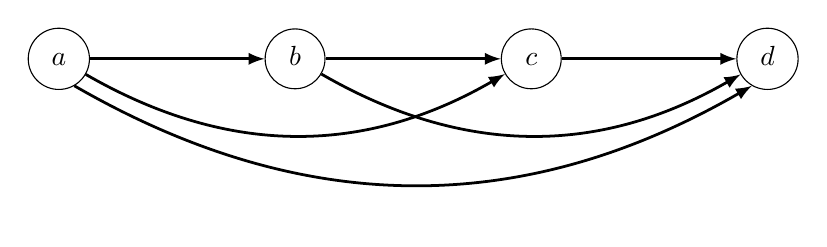
\begin{tikzpicture}[x=3cm,y=3cm]
        \begin{scope}[every node/.style={circle,draw}]
            \node (a) at (0,0) {\strut$a$};
            \node (b) at (1,0) {\strut$b$};
            \node (c) at (2,0) {\strut$c$};
            \node (d) at (3,0) {\strut$d$};
        \end{scope}
        \begin{scope}[line width=1pt,-latex]
            \draw (a.east)--(b.west);
            \draw (b.east)--(c.west);
            \draw (c.east)--(d.west);

            \draw (a.330) to[bend right] (c.210);
            \draw (a.300) to[bend right] (d.240);
            \draw (b.330) to[bend right] (d.210);
        \end{scope}
    \end{tikzpicture}
    \caption{Cascade form belief network}\label{Ch2Fig:4}
\end{figure}



\subsection{Markov chains}

A first order Markov Chain is depicted in the form of a belief network in Figure~\ref{Ch2Fig:5} and assumes that the immediate past is more relevant that the remote past in predicting the future. It specifies a joint probability distribution $p(v_1,\dots,v_T)$ over a collection of discrete or continuous variables. A first order Markov Chain is depicted in Figure~\ref{Ch2Fig:5}.

\begin{figure}[!ht]\centering
    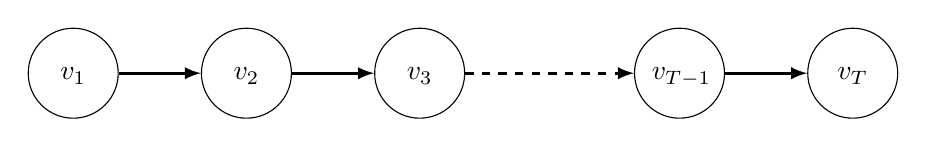
\begin{tikzpicture}[x=2.2cm,y=2cm,text width=20pt,align=center]
        \begin{scope}[every node/.style={circle,draw}]
            \node (v1)  at (1.0,0) {\strut$v_1$};
            \node (v2)  at (2.0,0) {\strut$v_2$};
            \node (v3)  at (3.0,0) {\strut$v_3$};
            \node (vt1) at (4.5,0) {\strut$v_{T-1}$};
            \node (vt)  at (5.5,0) {\strut$v_{T}$};
        \end{scope}
        \begin{scope}[line width=1pt,-latex]
            \draw (v1.east)--(v2.west);
            \draw (v2.east)--(v3.west);
            \draw[dashed] (v3.east)--(vt1.west);
            \draw (vt1.east)--(vt.west);
        \end{scope}
    \end{tikzpicture}
    \caption{First order Markov chain}\label{Ch2Fig:5}
\end{figure}

For a joint distribution of variables $v_1,...,v_T$ the following conditional probability relationship holds \autocite{barberBRML2012}
\begin{equation}
    p{(v_{1\text{:}T})} = p{(v_1)} p {(v_2|v_1)} p{(v_3|v_2)} \dots p{(v_T|v_{T-1})}
\end{equation}

This can be generalised to the form below:
\begin{equation}
    p{(v_1,\dots,v_T)} = p{(v_1)} \prod_{t=2}^{T} p {(v_t|v_{t-1})}
\end{equation}

\subsection{The hidden Markov model}

The Hidden Markov Model (HMM) is a tool for representing probability distributions over a sequence of observations. It has the following distinct properties \autocite{ghahramani2001introduction}:

\begin{enumerate}
  \item A visible observation at a particular time $t$ is generated by some underlying process whose state $H_t$ is `hidden' (or `latent') from the observer.
  \item There is an assumption that the hidden process satisfies a first order Markovian property: where given the value of $H_{t-1}$, the current state $H_t$ is independent of all the states prior to $t-1$. Therefore the state at a particular time $t$ captures everything we need to know about the history of the process in order to predict the future of the process \autocite{ghahramani2001introduction}. The visible variables $V_t$ also satisfy the Markov Property with respect to the hidden States, given $V_t$, $H_t$ is independent of the hidden states and visible variables at all other times.
\end{enumerate}

A first order HMM defines a Markov Chain on hidden variables $h_{1\text{:}T}$. Each observed (`visible') variable is dependent on the hidden variables through what is known as the `emission' distributions.

Figure~\ref{Ch2Fig:6} is a graphical model representing a HMM.

\begin{figure}[!ht]\centering
    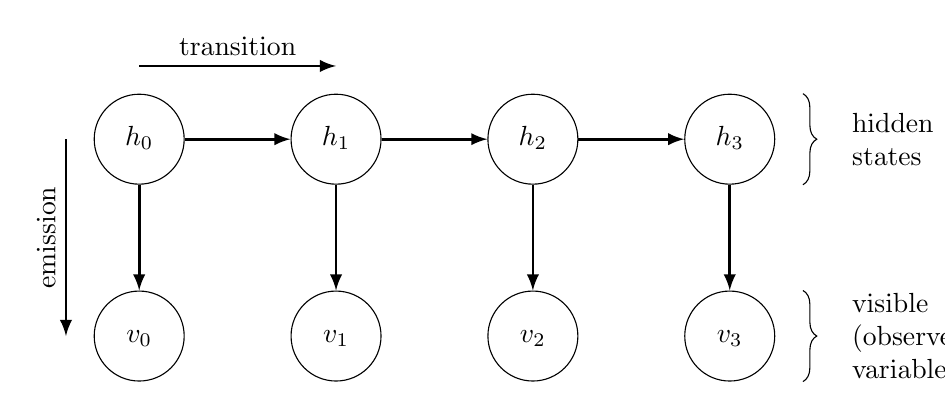
\begin{tikzpicture}[x=2.5cm,y=2.5cm]
        \begin{scope}[every node/.style={circle,draw,text width=20pt,align=center}]
            \node (h0)  at (0.0,1) {\strut$h_0$};
            \node (h1)  at (1.0,1) {\strut$h_1$};
            \node (h2)  at (2.0,1) {\strut$h_2$};
            \node (h3)  at (3.0,1) {\strut$h_3$};

            \node (v0)  at (0.0,0) {\strut$v_0$};
            \node (v1)  at (1.0,0) {\strut$v_1$};
            \node (v2)  at (2.0,0) {\strut$v_2$};
            \node (v3)  at (3.0,0) {\strut$v_3$};
        \end{scope}
        \begin{scope}[line width=1pt,-latex]
            \draw (h0.east)--(h1.west);
            \draw (h1.east)--(h2.west);
            \draw (h2.east)--(h3.west);
            \foreach \n in {0,1,2,3} {\draw (h\n.south)--(v\n.north);}
            \draw ([shift={(0pt,10pt)}]h0.north)coordinate(X) -- (h1.north|-X) node[midway,above] {transition};
            \draw ([shift={(-10pt,0pt)}]h0.west)coordinate(X) -- (v0.west-|X) node[midway,above,sloped,rotate=180] {emission};
        \end{scope}
        \draw [decorate,decoration={brace,amplitude=5pt}]
            ([shift={(10pt,0pt)}]h3.north-|h3.east) --
            ([shift={(10pt,0pt)}]h3.south-|h3.east)
            node [black,midway,right,xshift=0.5cm,text width=20pt] {hidden\\ states};
        \draw [decorate,decoration={brace,amplitude=5pt}]
            ([shift={(10pt,0pt)}]v3.north-|v3.east) --
            ([shift={(10pt,0pt)}]v3.south-|v3.east)
            node [black,midway,right,xshift=0.5cm,text width=20pt] {visible\\ (observed)\\ variables};
    \end{tikzpicture}
    \caption{Hidden Markov model with 4 hidden states}\label{Ch2Fig:6}
\end{figure}

The HMM Graphical model above Figure~\ref{Ch4Fig:3} above can be more generally written as a set of joint distributions below:
\begin{equation}
    p{(h_{0\text{:}T},v_{0\text{:}T})} =
    p{(v_0 | h_0)} \underbrace{p {(h_0)}}_{a}
    \prod_{t=1}^{T}
    \underbrace{p{(v_t | h_t)}}_{b}
    \underbrace{p {(h_t | h_{t-1})}}_{c}
\end{equation}
Where:
\begin{itemize}
    \item[$a$:] Is known as the prior
    \item[$b$:] Represents the emission distribution, more generally written as: $p{(v_t|h_t)}$
    \item[$c$:] Represents the transition distribution, more generally written: $p{(h_t|h_{t-1})}$
\end{itemize}

For discrete variables both the transition and emission distributions can be written in matrix form: a $H\times H$ matrix or the transition and $V\times H$ for the corresponding emission distribution. This matrix set-up and the format will be further discussed in the model set up for the RFQs.

At a high level a HMM is typically used to address 5 broad categories of inferential problems:

\begin{enumerate}
    \item \textbf{\textit{Filtering}} -- allows you to infer the present by obtaining the distribution of the hidden variable of interest ie $p{(h_t | v_{1\text{:}t})}$ using all the information up to the present $v_{1\text{:}t}$
    \item \textbf{\textit{Prediction}} -- $p{(h_t | v_{1\text{:}s})}$ inferring the future
    \item \textbf{\textit{Smoothing}} -- \textit{inferring the past} $p{(h_t | v_{1\text{:}u})}$
    \item \textbf{\textit{Likelihood}} -- \textit{used to establish the likelihood of a sequence of observations} $p{(v_{1\text{:}T})}$
    \item \textbf{\textit{Most likely Hidden Path}} -- \textit{this is known as the Viterbi Algorithm.}\\ $\argmax_{h_{1\text{:}T}} p{(h_{1\text{:}T} | v_{1\text{:}T})}$
\end{enumerate}


\subsection{Learning using the hidden Markov model}
\subsection{Expectation maximisation algorithm}

The Expectation Maximisation (EM) algorithm is a powerful iterative tool used to find maximising likelihood parameters when there is incomplete or missing data. This is very useful in real life examples where often we are faced with incomplete information. The EM algorithm applied to the HMM is known as the Baum-Welch \autocite{baum1970maximization} algorithm, but first we begin with the general form.

\subsubsection{General form}

To begin with we set this up as a belief network below where we have `visible' variables $v_n$ and a hidden (latent) variables $h_n$ which can be laid out per belief network in Figure~\ref{Ch2Fig:7} where $\harpoontheta$ is the collection of unknown parameters.

\begin{figure}[!ht]\centering
    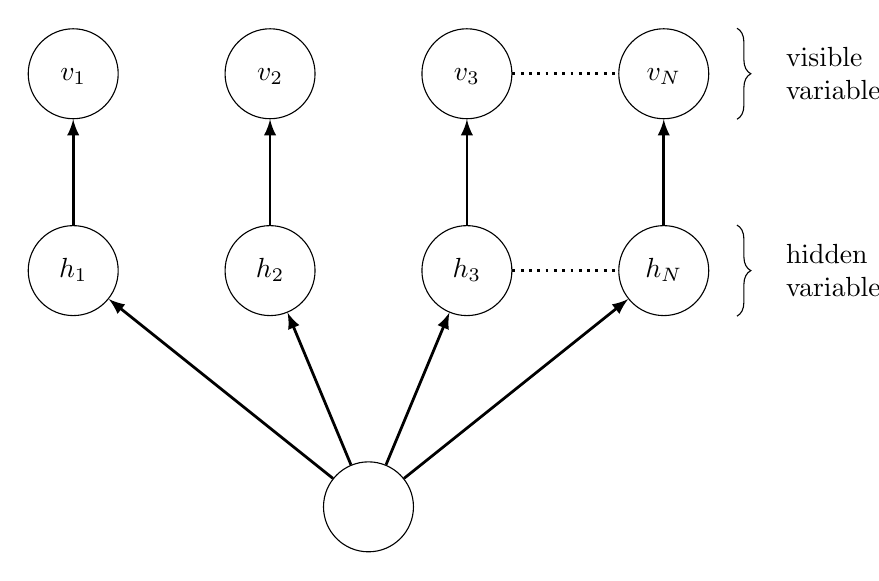
\begin{tikzpicture}[x=2.5cm,y=2.5cm]
        \begin{scope}[every node/.style={circle,draw,text width=20pt,align=center}]
            \node (v0)  at (0.0,1) {\strut$v_1$};
            \node (v1)  at (1.0,1) {\strut$v_2$};
            \node (v2)  at (2.0,1) {\strut$v_3$};
            \node (v3)  at (3.0,1) {\strut$v_N$};

            \node (h0)  at (0.0,0) {\strut$h_1$};
            \node (h1)  at (1.0,0) {\strut$h_2$};
            \node (h2)  at (2.0,0) {\strut$h_3$};
            \node (h3)  at (3.0,0) {\strut$h_N$};

            \node (t)  at (1.5,-1.2) {\strut$\harpoontheta$};

        \end{scope}
        \begin{scope}[line width=1pt,-latex]
            \foreach \n in {0,1,2,3} {\draw (h\n.north)--(v\n.south);
                \draw (t)--(h\n);}
            \foreach \n in {v,h} {\draw[dotted,-] (\n2.east)--(\n3.west);}
        \end{scope}
        \draw [decorate,decoration={brace,amplitude=5pt}]
            ([shift={(10pt,0pt)}]h3.north-|h3.east) --
            ([shift={(10pt,0pt)}]h3.south-|h3.east)
            node [black,midway,right,xshift=0.5cm,text width=20pt] {hidden\\ variables};
        \draw [decorate,decoration={brace,amplitude=5pt}]
            ([shift={(10pt,0pt)}]v3.north-|v3.east) --
            ([shift={(10pt,0pt)}]v3.south-|v3.east)
            node [black,midway,right,xshift=0.5cm,text width=20pt] {visible \\variables};
    \end{tikzpicture}
    \caption{Belief network for a collection of parameters with hidden and visible variables}\label{Ch2Fig:7}
\end{figure}

We can use `maximum likelihood' to find values of $\harpoontheta$ which maximise expression $p{(v_1,v_2,\dots,v_N| \harpoontheta)}$, where $v_n$ are actual values. That is another way of saying the most likely $\harpoontheta$ to have generated our data.

This objective is mathematically expressed as:
\begin{equation}
    \max_{\harpoontheta} p {(v_1,v_2,\dots,v_N | \harpoontheta)}
\end{equation}

Which given the $v_n$ are independent given $\harpoontheta$
\begin{equation}
    \max_{\harpoontheta} {( p{(v_1|\harpoontheta)}\cdot p{(v_2|\harpoontheta)} \cdot \dots \cdot p{(v_N| \harpoontheta)} )}
\end{equation}

We can evaluate each term using the below expression:
\begin{equation}
    p{(v_1|\harpoontheta)} = \sum_{h_i} p {(v_i,h_i | \harpoontheta)} =
        \sum_{h_i} p {(v_i | h_i)} p {(h_i | \harpoontheta)}
\end{equation}

However maximising the overall expression below is difficult due to the summation and as such there is no closed form solution.
\begin{equation}\label{Expre1}
    p{(v_1,v_2,\dots,v_N | \harpoontheta)} = \sum_{h_i,\dots,h_n} p {(v_1,\dots,v_N,h_i,\dots,h_N | \harpoontheta)}
\end{equation}

Therefore we use our iterative tool the EM algorithm. We do not directly maximise (\ref{Expre1}) but we maximise a lower bound, which effectively pushes (\ref{Expre1}) into its maximum. This is repeated as a two-step process.

Lets call $p {(v_1,\dots,v_N,h_i,\dots,h_N | \harpoontheta)} \rightarrow p{(\harpoon{v},\harpoon{h} | \harpoontheta)}$ i.e. $v$ and $h$ vectors are gathered together. We also need to define a second probability distribution $q$ which is what we need to change in each step.

Next, consider the Kullback-Leibler (KL) divergence expression below:
\begin{equation}
    \KL ( q{(\harpoon{h}|\harpoon{v})},p{(\harpoon{h}|\harpoon{v},\harpoontheta)} )
\end{equation}

And as we know $\KL$ divergences are always non-negative (a proof for this provided in the Appendix~\ref{AppA} as this is property is widely used), we therefore we have the expression below:
\begin{equation}
    \KL {( q{(\harpoon{h}|\harpoon{v})},p{(\harpoon{h}|\harpoon{v},\harpoontheta)} )}\geq 0
\end{equation}

Which can be expanded out to the form below (\ref{Equation3})
\begin{equation}\label{Equation3}
    {\left\langle \log q {(\harpoon{h}|\harpoon{v})}\right\rangle}_{q{(\harpoon{h}|\harpoon{v})}} -
    {\left\langle\log p {(\harpoon{h}|\harpoon{v},\harpoontheta)}\right\rangle}_{q{(\harpoon{h}|\harpoon{v})}}
    \geq 0
\end{equation}

And given the 3 statements below:
\begin{gather}
    p {(\harpoon{h}|\harpoon{v},\harpoontheta)} = 
        \dfrac{ p {(\harpoon{h},\harpoon{v}|\harpoontheta)}}
              { p {(\harpoon{v}|\harpoontheta)}} \\
    \log {\left(\dfrac{a}{b}\right)} = \log a - \log b \\
    {\left\langle a-b \right\rangle}_{q} = {\left\langle a \right\rangle}_{q} - {\left\langle b \right\rangle}_{q}
\end{gather}

Expression~(\ref{Equation3}) can be re-written as:
\begin{equation}
    {\left\langle \log q (\harpoon{h},\harpoon{v}) \right\rangle}_{q} -
    {\left\langle \log p (\harpoon{h},\harpoon{v}|\harpoontheta) \right\rangle}_{q} +
    {\left\langle \log p (\harpoon{h}|\harpoontheta) \right\rangle}_{q}
    \geq 0
\end{equation}

Where for convenience $q$ represents a short-hand for $q( \harpoon{h}|\harpoon{v} )$. We can re-arrange the above expression to give:
\begin{equation}
    \underbrace{{\left\langle \log p (\harpoon{v}|\harpoontheta) \right\rangle}_{q}}_{a}
    \geq
    {\left\langle \log p (\harpoon{h},\harpoon{v}|\harpoontheta) \right\rangle}_{q} -
    {\left\langle \log q (\harpoon{h}|\harpoon{v}) \right\rangle}_{q}
\end{equation}

The first term ($a$) in the preceding expression equates to $p (\harpoon{v}|\harpoontheta)$ as there is no $q$ distribution term inside $\langle\cdots\rangle$ and the expectation with respect to $q$ has no impact, thus resulting in the expression~(\ref{Eq:4.18}):
\begin{equation}\label{Eq:4.18}
    {p (\harpoon{v}|\harpoontheta)}_{q}
    \geq
    \underbrace{{\left\langle \log p (\harpoon{h},\harpoon{v}|\harpoontheta) \right\rangle}_{q}}_{\text{known as the ``Energy'' term}}
    -
    \underbrace{{\left\langle \log q (\harpoon{h}|\harpoon{v}) \right\rangle}_{q}}_{\text{known as the ``Entropy'' term}}
\end{equation}

Therefore if we can manipulate and maximise the right hand side of the expression above because of the ``$\geq$'' term we effectively maximise the left hand side also. To maximise the right hand side we use the EM algorithm.

We choose any initial values for our parameters in $\harpoontheta$, then keep repeating the E-step followed by the M-Step below until $\harpoontheta$ stops changing and you end up with final values of $\harpoontheta$.

\begin{description}
    \item[E-Step] -- Let each $q(h_n|v_n) = p ( h_n | v_n,\harpoontheta )$
    \item[M-Step] -- update $\harpoontheta$ by choosing $\harpoontheta$ that maximises the energy term.
\end{description}

\subsection{Baum-Welch algorithm}

The Baum-Welch algorithm \autocite{baum1970maximization} represents the application of the EM algorithm to the HMM model.

Given a set of data the algorithm helps us find the HMM emission matrix $B$ and transition matrix $A$ and an initial vector $a$ which is most likely to have generated our data set 
$\mathcal{V}=\left\{\mathbf{v}^1,\dots,\mathbf{v}^N\right\}$
where
$\mathbf{v}^n = v^{n}_{1\text{:$T_n$}}$ is of length $T_n$.

The assumptions for application of Baum-Welch are that dataset $V$ is comprised of discrete (i.e. not continuous set of variables). It is also assumed that the number of both hidden (H) and visible (V) variables is known, and each sequence was generated as independent and identically distributed random variables (IID).

The Baum-Welch follows the form described earlier in the section on General Form EM Algorithm more specifically with M and E steps below \autocite{barberBRML2012}

\begin{description}
    \item[M-Step] -- The `energy' term is maximised with respect to the transition matrix ($A$), emission matrix ($B$) as well as the hidden states $h_{1\text{:$T_n$}}$ ($\mathbf{h}^n$) and the initial vector $a$.
\end{description}

\begin{equation}
    \sum_{n=1}^{N} {
        \left\langle \log p
            (
                v_1^n,v_2^n,\dots,v_{\text{$T^n$}}^n,h_1^n,h_2^n,\dots,h_{\text{$T^n$}}^n
            )
        \right\rangle
        }_{p^{\text{old}} (\mathbf{h}^n|\mathbf{v}^n)}
\end{equation}

Applying the HMM structure to the above we obtain:

\begin{equation}
    \sum_{n=1}^{N} \left\{
        {\left\langle\log p (h_1)\right\rangle}_{p^{\text{old}} (h_1^n|\mathbf{v}^n)}
        +
        \sum_{t=1}^{T_n - 1}
        {\left\langle \log p ( h_{t+1}|h_t ) \right\rangle}_{p^{\text{old}} (h_t,h_{t+1}|\mathbf{v}^n)}
        +
        \sum_{t=1}^{T_n}
        {\left\langle \log p ( v_t^n | h_t ) \right\rangle}_{p^{\text{old}} (h_t,|\mathbf{v}^n)}
    \right\}
\end{equation}

The probability that first hidden variable is in a state $i$ can be expressed as $p^{\text{new}} (h_1=i)$ and optimising the above expression [xx] by making $p(h_1)$ to be a distribution and avoiding the sequencing of $h$ variables index we obtain:

\begin{equation}\label{Eq:4.22}
    a_i^{\text{new}} \equiv p^{\text{new}} (h_1=i) = \dfrac{1}{N}
    \sum_{n=1}^{N} p^{\text{old}} (h_1=i|\mathbf{v}^n )
\end{equation}

This can be further written as per below which is the number of times on average the first hidden variable is in a particular state $i$

\begin{equation}\label{Eq:4.23}
    A_{i^\prime,i}^{\text{new}}\equiv
    p^{\text{new}}
    ( h_{t+1} = i^\prime | h_t = i )
    \propto
    \sum_{n=1}^{N}
    \sum_{t=1}^{T_{n-1}}
    p^{\text{old}} ( h_t = i,h_{t+1} = i^\prime|\mathbf{v}^n )
\end{equation}

If we normalise the above expression using a normalisation constant in the denominator. Basically how many times do we transition from one state ($i$) to another state $i^\prime$

\begin{equation}\label{Eq:4.24}
    A_{i^\prime,i}^{\text{new}} =
    \dfrac
        {
            \sum_{n=1}^{N}
            \sum_{t=1}^{T_n -1}
            p^{\text{old}} ( h_t = i,h_{t+1} = i^\prime|\mathbf{v}^n )
        }
        {
            \sum_{i^\prime}
            \sum_{n=1}^{N}
            \sum_{t=1}^{T_n -1}
            p^{\text{old}} ( h_t = i,h_{t+1} = i^\prime|\mathbf{v}^n )
        }
\end{equation}

We can then perform the M-Step for the emission from hidden states to visible below. This is effectively expectation of the number of times the visible variable is in a state $j$ and the hidden in a state $i$ (the normalisation constant is replaced with the proportional symbol).

\begin{equation}\label{Eq:4.25}
    B_{j,i}^{\text{new}} \equiv p^{\text{new}} ( v_t = j| h_t = i )
    \propto
    \sum_{n=1}^{N}
    \sum_{t=1}^{T_n}
    ||
    \left[v_t^n = j\right]
    p^{\text{old}} (h_t = i|\mathbf{v}^n)
\end{equation}

\begin{description}
    \item[E-Step] -- The smoothing inference method described earlier ($p(h_t|v_{1\text{:}u})$) is used to obtain the expression below. The solution then involves repeating (\ref{Eq:4.22}), (\ref{Eq:4.24}), and (\ref{Eq:4.25}) above until convergence where the algorithm converges to a maximum likelihood note this may not be the global maximum and it turns out the initialisation of the emission distribution is key.
\end{description}
\begin{gather}
    p^{\text{old}} ( h_1 = i|\mathbf{v}^n ) \\
    p^{\text{old}} ( h_t = i,h_{t+1} = i^\prime | \mathbf{v}^n ) \\
    p^{\text{old}} ( h_t = i|\mathbf{v}^n )
\end{gather}


\section{Artificial neural networks}

\subsection{Background and Applications}

The first mathematical model of artificial neurons was introduced in 1943 by McCulloch and Pitts \autocite{mcculloch1943logical}. The idea was further developed by Franck Rosenblatt who in 1958 introduced the concept of a perceptron (generic name given to artificial neural networks) algorithm \autocite{rosenblatt1958perceptron}

Artificial neural networks (ANNs) are powerful, layered machine learning models, which attempt to computationally model the information processing abilities of biological neurons in our brains. There are many types of ANNs, to name a few feed-forward neural networks (NNs), convolutional neural networks and recurrent neural networks. This introduction will focus mainly on feed-forward neural networks which are the most common type of NN, for example MLPRegressor in the popular python library scikit-learn.

Neural Networks have a wide range of applications in the real world, to name a few:
\begin{description}
    \item[Image recognition] -- Geoff Hinton et al \autocite{krizhevsky2012imagenet} use deep convolutional neural networks (CNNs) to successfully classify 1.2million images into 1,000 different classes from the ImageNet data-set with record breaking low error rates compared to previous attempts.
    \item[Medicine] -- Neural networks (NNs) have been applied successfully in disease diagnosis. An application of NNs has been in Urology where specialists are often faced with difficulties in obtaining a correct diagnosis. This is mainly due to the multiple complex variables involved in urological dysfunctions. David Gil et al \autocite{gil2009application} successfully used multilayer perceptron trained with backpropagation to help urologists make more accurate diagnoses.
    \item[Time-series prediction] -- Neural networks (NNs) have been widely used to model time-series data in a variety of fields but in particular finance and economics. Huang et al \autocite{huang2004credit} used backpropogation NNs to successfully model and predict corporate credit ratings for the Taiwan and US markets making such information more accessible to investors.
    \item[Natural language processing (NLP)] -- NNs have helped to solve many problems in this area with applications in text classification, part of speech tagging, character recognition, spell checking and machine translation. Sebastien Riedel and Tim Rockt\"aschel \autocite{rocktaschel2017end} recently used neural networks to infer facts from a given knowledge base. This has enabled automation completion of large Knowledge Bases by establishing complex reasoning patterns based on similarities.
\end{description}



\subsection{Feed-forward neural networks}\label{feedfwdnn}

Feed-forward Neural Networks (also referred to as deep forward neural networks or multilayer perceptrons (MLPs)) are very common and primarily used for supervised learning.

Figure~\ref{Ch2Fig:8} depicts a typical graphical architecture for a feed-forward neural network where the circles represent neurons. The input layer information $x_1\text{:}x_3$, which needs to be evaluated, flows forward through the one hidden layer to the output layer $y_1\text{:}y_2$. They are called feed-forward, as there are no feedback connections where output information is fed back on itself into the network. There are weights and bias parameters assigned to each arrow, which are typically initialised to a small random value as the start.

\begin{figure}[!ht]\centering
    \begin{tikzpicture}[x=4cm,y=1.5cm]
        \begin{scope}[
            every node/.style={circle,draw,text width=10pt,align=center,fill=black!50},
            cx/.style={fill=COL1},
            cy/.style={fill=COL2},
            cc/.style={fill=black!20},
        ]
            \node[cx] (x1)  at (1,1)   {\strut$x_1$};
            \node[cx] (x2)  at (1,0) {\strut$x_2$};
            \node[cx] (x3)  at (1,-1)  {\strut$x_3$};
            %
            \node[cy] (y1)  at (3,0.5) {\strut$y_1$};
            \node[cy] (y2)  at (3,-0.5) {\strut$y_2$};
            %
            \node[cc] (c1)  at (2, 1.5) {\strut};
            \node[cc] (c2)  at (2, 0.5) {\strut};
            \node[cc] (c3)  at (2,-0.5) {\strut};
            \node[cc] (c4)  at (2,-1.5) {\strut};
            %
        \end{scope}

        \begin{scope}[thin,-latex]
            \foreach \x in {1,...,3} {
                \draw[latex-] (x\x.west)--++(180:0.5);
                \foreach \c in {1,...,4} {\draw (x\x) -- (c\c);}
            }
            \foreach \c in {1,...,4} {
                \foreach \y in {1,...,2} {
                    \draw (y\y.east)--++(0:0.5);
                    \draw (c\c) -- (y\y);
                }
            }
        \end{scope}

        \coordinate (B) at (1,-2);
        \coordinate (T) at (1,2);
        \coordinate (A) at (1,2.7);
        \draw [decorate,decoration={brace,amplitude=5pt,mirror}] (B-|x1.west) -- (B-|x1.east) node [midway,below,yshift=-5pt,align=center,font=\footnotesize] {inputs};
        \draw [decorate,decoration={brace,amplitude=5pt,mirror}] (B-|c1.west) -- (B-|c1.east) node [midway,below,yshift=-5pt,align=center,font=\footnotesize,text width=1cm,align=center] {hidden\\ layer};
        \draw [decorate,decoration={brace,amplitude=5pt,mirror}] (B-|y1.west) -- (B-|y1.east) node [midway,below,yshift=-5pt,align=center,font=\footnotesize] {outputs};
        %
        \draw [decorate,decoration={brace,amplitude=5pt,mirror}] ([xshift=4pt]B-|x1.east) -- ([xshift=-4pt]B-|c1.west) node [midway,below,yshift=-5pt,align=center,font=\footnotesize] {weights (W)};
        \draw [decorate,decoration={brace,amplitude=5pt,mirror}] ([xshift=4pt]B-|c1.east) -- ([xshift=-4pt]B-|y1.west) node [midway,below,yshift=-5pt,align=center,font=\footnotesize] {weights (W)};
        %
        \draw[-latex] (T-|x1.east)--(T-|y1.west) node[midway,above,font=\footnotesize\bfseries]{feed-forward};
    \end{tikzpicture}
    \caption{Example high-level architecture for a feed-forward neural network with 3 inputs and 2 outputs}\label{Ch2Fig:8}
\end{figure}

Figure~\ref{Ch2Fig:9} below is a simple feed-forward neural network with 1 input vector $\mathbf{x_1}$ and 1 hidden layer. The predicted output y is produced as a result of feeding $x$ input(s) through the hidden layers and eventually it translates to a loss or cost function when compared with the actual value.

\begin{figure}[!ht]\centering
    \strut\\
    \resizebox{\linewidth}{!}{\begin{tikzpicture}[x=2.2cm,y=1cm]
        \node[inner sep=1pt,circle,draw=black,fill=COL1] (N11) at (0,0) {\strut$x$};
        \begin{scope}[every node/.style={inner sep=1pt,anchor=west,font=\small}]

            \node[circle,draw] (N21) at ([xshift=1.0cm]N11.east) {\strut$m_1$};
            \node (N22) at (N21.east) {\strut$x$};
            \node (N23) at (N22.east) {\strut$+$};
            \node[circle,draw] (N24) at (N23.east) {\strut$c_1$};

            \node (N31) at ([xshift=1.0cm]N24.east) {\strut ReLU};

            \node[circle,draw] (N41) at ([xshift=1.0cm]N31.east) {\strut$m_2$};
            \node (N42) at (N41.east) {\strut$x$};
            \node (N43) at (N42.east) {\strut$+$};
            \node[circle,draw] (N44) at (N43.east) {\strut$c_2$};

            \node (N51) at (4.5,-1) {$\hat{y}$};
            \node[anchor=north] (N52) at ([yshift=-5pt]N51.south) {\phantom{$y$}};% THIS
            \node[inner sep=3pt,circle,draw=black,fill=COL1] (yyy) at (N44.west|-N52) {$y$};
            \draw[-latex] (yyy)--([shift={(-6pt,0pt)}]N52.west) coordinate[midway](yyym);
            \coordinate (N53) at ($(N51)!0.5!(N52)$);

            \node[rectangle,draw,inner sep=4pt,text=COL3,fill=COL1,draw=black] (N61) at ([xshift=1cm]N53) {loss $\mathscr{L}=e^2$};
            \node[text=COL3] (N71) at ([xshift=1.5cm]N61) {$\mathscr{L}$};
        \end{scope}

        \begin{scope}[-latex]
            \draw ([shift={(5pt,0pt)}]N11.east) -- ([shift={(-8pt,0pt)}]N21.west);
            \draw ([shift={(5pt,0pt)}]N24.east) -- ([shift={(-8pt,0pt)}]N31.west);
            \draw ([shift={(8pt,0pt)}]N31.east) -- ([shift={(-8pt,0pt)}]N41.west);
            \draw ([shift={(11pt,0pt)}]N53) -- ([shift={(-1pt,0pt)}]N61.west) coordinate[pos=0.5](yy);
            \draw ([shift={(2pt,0pt)}]N61.east) -- ([shift={(-1pt,0pt)}]N71.west);
            \draw ([shift={(4pt,6pt)}]N44.east) --++ (10pt,0pt) coordinate(N4151) -- (N4151|-N51.west) coordinate[pos=0.2](ev) -- ([shift={(-6pt,0pt)}]N51.west);
            %\draw ([shift={(4pt,-6pt)}]N44.east) --++ (5pt,0pt) coordinate(N4152) -- (N4152|-N52.west) -- ([shift={(-6pt,0pt)}]N52.west);
        \end{scope}

        \begin{scope}[every node/.style={at end,above,font=\footnotesize}]
            \draw (N11.north)--++(90:0.8) coordinate (X) node {\strut input};
            \draw (N21.north)--(N21|-X) node {\strut weights};
            \draw (N24.north)--(N24|-X) node {\strut bias};
            \draw (N31.north)--(N31|-X) node {\strut non-linearity};
            \draw (N41.north)--(N41|-X) node {\strut weights};
            \draw (N44.north)--(N44|-X) node {\strut bias};
            \draw (ev)--++(10pt,0pt)--++(90:40pt)--++(0:50pt) coordinate (EV) node[at end,right,text width=2.5cm] {estimated value\\ (output)};

            \draw (yy)--++(90:40pt) coordinate(yy1)--(yy1-|EV) coordinate (YY) node[at end,right] {$\hat{y}-y$ \textcolor{COL3}{(error $(e)$)}};
            \draw (yyym)--++(270:0.8) node[below]{actual value};
        \end{scope}

        \draw[-latex] (0.5,2.2) --++(0:4cm) node[midway,above,font=\small\bfseries] {Feed-forward};
        \draw[-latex] (3.5,-2.6) --++(180:4cm) node[midway,above,font=\small\bfseries] {Back- propagation};

        \begin{scope}[on background layer]
            \fill[COL1,draw=black] ([shift={(-6pt,-6pt)}]N21.south west) rectangle ([shift={(6pt,6pt)}]N24.north east);
            \fill[COL1,draw=black] ([shift={(-6pt,-6pt)}]N31.south west) rectangle ([shift={(6pt,6pt)}]N31.north east);
            \fill[COL1,draw=black] ([shift={(-6pt,-6pt)}]N41.south west) rectangle ([shift={(6pt,6pt)}]N44.north east);
            \fill[COL1,draw=black] ([shift={(-6pt,-6pt)}]N52.south west) rectangle ([shift={(6pt,6pt)}]N51.north east);
        \end{scope}
    \end{tikzpicture}}
    \caption{Example of a feed-forward neural network with labelled components}\label{Ch2Fig:9}
\end{figure}

The total error of the network is called the loss (or cost) function $L$, which measures the difference between the actual and predicted values. The objective is to minimise this loss, which is a mean squared error (MSE) of the general form below:
\begin{equation}
    \mathscr{L} = \dfrac{1}{n} \sum_{i=1}^{n} {\left( {y}^{(i)} - {\hat{y}}^{(i)} \right)}^{2}
\end{equation}

The `squared' loss function is smooth and is differentiable, which is necessary for back-propagation. The chain rule is used to calculate the derivative of the loss function with respect to the weights and bias term.

Rather than focusing on the individual neurons, nowadays feed-forward neural networks are more commonly thought of as using the framework of linear algebra.

Sets of variables at each layer of the network can be represented in vector form, and the linear multiplication layers can be represented as matrix multiplications. This view also has the advantage in that it allows neural network training and prediction calculations to be performed efficiently and at scale making use of already-existing linear algebra software libraries.

The number of hidden layers determines the ``depth'' of the model and the existence of more that one hidden layer has lead to the term ``deep'' neural networks or ``deep learning''.

In designing a neural network one should consider the number of hidden layers as well as the type of `activation function' to calculate the hidden layer values.

The component ReLU stands for rectified linear unit and is the most common `activation functions' used in feed-forward neural networks. Other activation functions such as sigmoid or Tanh can also be used in NNs. ReLU is in fact a non-linear function, for example a given input $x$ and output $y$ (Figure~\ref{Ch2Fig:10}) can be represented by Expression~\ref{Ch2Eq2.36} and the line plot in Figure~\ref{Ch2Fig:11}.

\begin{figure}[!ht]\centering
    \strut\\
    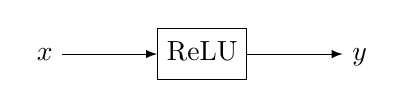
\begin{tikzpicture}[x=2cm,y=2cm]
        \node (N1) at (0,0) {\strut$x$};
        \node[rectangle,draw] (N2) at (1,0) {\strut ReLU};
        \node (N3) at (2,0) {\strut$y$};

        \draw[-latex] (N1.east)--(N2.west);
        \draw[-latex] (N2.east)--(N3.west);
    \end{tikzpicture}
    \caption{Non-linear rectified linear unit block with input and output}\label{Ch2Fig:10}
\end{figure}

We end up with the mathematical relationship below as a result of ReLU transformation:

\begin{equation}\label{Ch2Eq2.36}
    y(x) = \left\{
        \begin{array}{ll}
            x & \text{$x\geq0$} \\
            0 & \text{otherwise}
        \end{array}\right.
\end{equation}

\begin{figure}[!ht]\centering
    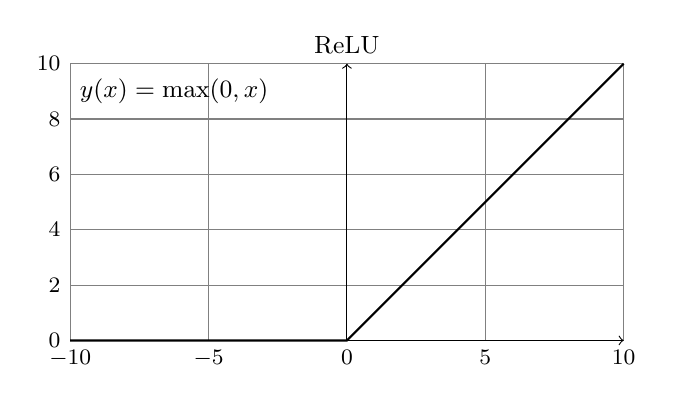
\begin{tikzpicture}[x=10pt,y=10pt]
        \foreach \x in {-10,-5,0,5,10} {
            \draw[black!50,thin] (\x,0)--(\x,10);
            \node[below,font=\footnotesize] at (\x,0) {$\x$};
        }

        \foreach \y in {0,2,4,6,8,10} {
            \draw[black!50,thin] (-10,\y)--(10,\y);
            \node[left,font=\footnotesize] at (-10,\y) {$\y$};
        }
        \draw[->] (0,0) -- (10,0);
        \draw[->] (0,0) -- (0,10);

        \draw[thick] (-10,0)--(0,0)--(10,10);

        \node[above,font=\small] at (0,10) {ReLU};
        \node[right,font=\small] at (-10,9) {$y(x)=\max (0,x)$};

    \end{tikzpicture}
    \caption{Line plot of ReLU}\label{Ch2Fig:11}
\end{figure}


ReLU plays an important role in the NN architecture, as without it the network ends up being a bunch of cascaded linear functions which overall are still linear and thus unable to fit well to complex data sets. Therefore the non-linearity is an important property of the network, which also helps to deal with large spread of input values.

The back-propagation algorithm is used to compute the gradients of functions in our network. The purpose of back-propagation is to update the assigned weights in our neural network such that the overall NN loss is minimised. So the partial derivative of the loss is obtained with respect to all parameters (namely the weights and bias terms). Once these as known we use gradient descent to update the values. For example one such update for weight $m_1$ is shown below with learning rate $\alpha$ which is a constant.

\begin{equation}
    m \leftarrow m_1-\alpha \dfrac{\partial L}{\partial m_i}
\end{equation}

As a side note, Goodfellow et al \autocite{rosenblatt1958perceptron} point out the term back-propagation is often misquoted to be the entire learning algorithm for multilayer neural networks, whereas in fact it refers to a method for computing the gradient while an iterative algorithm such as stochastic gradient descent (SGD) is used to perform learning using this gradient to in order to minimise the loss value.